\chapter{Modelling} \label{chp:models}
    Although the work of this project was primarily experimental, some modelling work was performed in order to better understand the physics of LSP and aid in the experimental design. One major area of interest is in determining the absorption properties of LSP. High laser absorption is desirable to maximize power conversion efficiency. Furthermore, the IB absorption coefficient typically reaches a maximum at a specific temperature. According to \textcite{keeferLaserSustainedPlasmas1989}, this peak absorption temperature was found to closely correlate with LSP peak temperature. The measurement of absorption coefficient can thus be used to support LSP temperature estimates.

    \section{Absorption} \label{sec:models_absorption}
        A critical property of LSP is its ability to absorb laser radiation. As stated in \autoref{sec:background_lsp}, the primary mechanism for radiation absorption in LSP is inverse bremsstrahlung. Calculation of the absorption coefficient of this process is critical for modelling LSP behavior and estimating its laser absorption efficiency. The calculation method presented here aims to adapt the work of \textcite{akarapuNumericalModelLasersustained2009,nassarInvestigationLasersustainedPlasma2012}, who have developed CFD models for the use of argon LSP in surface-treatment applications. Although their work considered \ce{CO_2} lasers, adapting the method to the fiber laser of this study is a matter of using the appropriate laser frequency in \autoref{eq:ib_absorption}. Their work was thus used to validate each calculation step, and their results will be plotted alongside this study's computations when relevant. \added{A step-by-step example calculation is provided in \autoref{sec:app_calc_ex_alpha}.}
        
        The absorption coefficient can be calculated using \autoref{eq:ib_absorption} and is heavily dependent on electron density $n_\mathrm{e}$ and radiation frequency $\nu$. The first step of absorption modelling is thus to determine electron density, which is variable with temperature $T$ according to the Saha ionization equation, developed by \textcite{sahaPhysicalTheoryStellar1997}. It is reproduced here for the single ionization case as \autoref{eq:saha}.
        \begin{equation}
            \frac{n_\mathrm{e}^2}{n_0-n_\mathrm{e}} = \frac{n_\mathrm{e}^2}{n_\mathrm{Ar}} = \frac{2}{\Lambda_\mathrm{th}^3}\frac{\mathcal{Z}_{\mathrm{Ar}^+}}{\mathcal{Z}_\mathrm{Ar}}\exp{\left(-\frac{E_\text{ion, Ar}}{k_\mathrm{B}T}\right)}
            \label{eq:saha}
        \end{equation}
        Where $n_0$ is the initial number density of neutral atoms, $n_\mathrm{Ar}$ is the number density of un-ionized atoms at a given temperature, $E_\text{ion, Ar}$ is argon's first ionization energy (\qty{15.76}{eV}~\cite{liasIonizationEnergyEvaluation2023}), and $k_\mathrm{B}$ is the Boltzmann constant. \added{In this case, the product $k_\mathrm{B}T$ can be expressed in J or eV depending on the unit of $E_\text{ion, Ar}$. }The thermal DeBroglie wavelength $\Lambda_\mathrm{th}$ is a function of temperature as follows, where $\hbar$ is the reduced Planck constant and $m_\mathrm{e}$ is the mass of an electron:
        \begin{equation*}
            \Lambda_\mathrm{th} = \sqrt{\frac{2\pi \hbar^2}{m_\mathrm{e}k_\mathrm{B}T}}
        \end{equation*}
        The ratio $\mathcal{Z}_{\mathrm{Ar}^+}/\mathcal{Z}_\mathrm{Ar}$ is the ratio of the partition function values for Ar$^+$ and Ar (also designated Ar II and Ar I, respectively). These values are also dependent on temperature and can be queried in the NIST Atomic Spectra Database (ASD) (\textcite{kramidaNISTAtomicSpectra2022}) for a given spectrum (e.g., Ar I) and electron temperature $T_\mathrm{e}$. This ratio is plotted in \autoref{fig:e_density_partition}. \citeauthor{nassarInvestigationLasersustainedPlasma2012} fitted a seventh-order polynomial (shown in \autoref{eq:nassar_polynomial}) to approximate this ratio across temperature\added{:
        \begin{multline} \label{eq:nassar_polynomial}
            \frac{\mathcal{Z}_{\mathrm{Ar}^+}}{\mathcal{Z}_\mathrm{Ar}} = -2.3077\times 10^{-29}T^7+2.3474\times 10^{-24}T^6 \\ - 8.8453\times 10^{-20}T^5
            + 1.4851\times 10^{-15}T^4 -9.843\times 10^{-12}T^3\\ - 1.2477\times 10^{-8}T^2
            + 0.00047534T+3.7971
        \end{multline}
        This approximation is plotted alongside the data directly retrieved from the NIST ASD in \autoref{fig:e_density_partition} for comparison.}

        It is important to note that $n_0$ in \autoref{eq:saha} is not constant across temperatures. In the case of LSP, the ionization process occurs at constant pressure, even if the experiment occurs in a closed container, as only a small fraction of the test section volume undergoes ionization. The hotter argon is free to expand into the cooler surroundings, locally reducing the number density and maintaining a constant pressure. Therefore, $n_0$ must be calculated based on a given pressure $p$ and the varying temperature. This can be done with the ideal gas equation, where $V$ is volume, $N$ is the number of atoms in moles, $R_\mathrm{u}$ is the universal gas constant, and $N_\mathrm{A}$ is Avogadro's number:
        \begin{align*}
            pV&= NR_\mathrm{u}T \\
            p&= \frac{N}{V}R_\mathrm{u}T \\
            \frac{N_\mathrm{A}p}{R_\mathrm{u}T}&= n_0
        \end{align*}

        The electron density $n_\mathrm{e}$ is plotted against temperature in \autoref{fig:e_density_curves}, for a pressure of \qty{1}{bar}. The calculation by \citeauthor{nassarInvestigationLasersustainedPlasma2012} is plotted alongside it, and their relative value is compared. While the electron density plots appear to agree, there remains a difference in density of a factor of two. This appears to be due to the use of lower precision physical constants in \citeauthor{akarapuNumericalModelLasersustained2009} and \citeauthor{nassarInvestigationLasersustainedPlasma2012}'s work.

        \begin{figure}[h]
            \centering
            \begin{subfigure}[t]{2.6in}
                \centering
                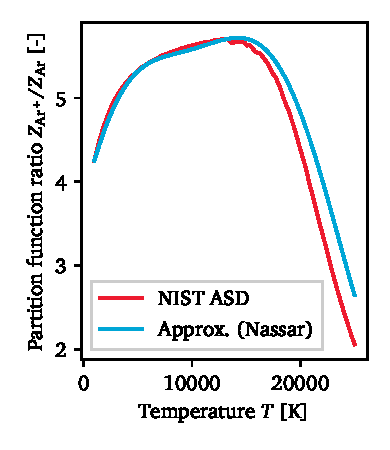
\includegraphics[]{assets/4 models/partition}
                \caption{Ratio of Ar II to Ar I partition function values}
                \label{fig:e_density_partition}
            \end{subfigure}
            \hfill
            \begin{subfigure}[t]{3.2in}
                \centering
                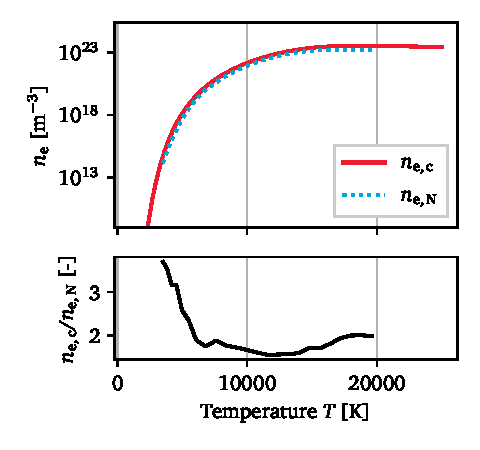
\includegraphics[]{assets/4 models/n_e}
                \caption{$n_\mathrm{e}$ at \qty{1}{bar}, and comparison between computed density $n_\mathrm{e, c}$ and density $n_\mathrm{e, N}$ reported by \textcite{nassarInvestigationLasersustainedPlasma2012}}
                \label{fig:e_density_curves}
            \end{subfigure}
            \caption{Computation of electron density $n_\mathrm{e}$ of argon}
            \label{fig:e_density}
        \end{figure}

        Although electron density appears to plateau past \qty{20000}{K}, the caveat of this calculation is that it only considers single-ionization, i.e., removing a single electron from the atom. While this is valid below \qty{20000}{K}, second-degree ionization (removing a second electron away) begins past this temperature, increasing the number of electrons in the plasma. The plot is extended up to \qty{25000}{K} to provide some estimate of plasma properties, although they will not be as accurate as below \qty{20000}{K}.

        The absorption coefficient $\alpha$ can now be calculated with the known electron density. For convenience, the equation for $\alpha$, \autoref{eq:ib_absorption}, is reproduced here:
        \begin{equation*}
            \ibalphaeq \tag{\ref{eq:ib_absorption} revisited}
        \end{equation*}
        Most parameters have been defined in \autoref{sec:background_lsp}, so the Coulomb logarithm $\ln{\Lambda}$ and the plasma frequency $\nu_\mathrm{p}$ will be of interest here. The Coulomb logarithm is evaluated by \textcite{nassarInvestigationLasersustainedPlasma2012} using a common approximation seen in plasma physics (\textcite{richardson2019NRLPlasma2019}):
        \begin{equation}\label{eq:coulombLog_NRL}
            \ln{\Lambda} \approx 23-\ln{(n_\mathrm{e}^{1/2}ZT_\mathrm{e}^{-3/2})}
        \end{equation}
        However, alternate evaluations of the logarithm exist, such as the one given by \textcite{johnstonCorrectValuesHighfrequency1973} in the specific context of IB absorption coefficient calculation (\autoref{eq:coulombLog_johnston}). 
        \begin{equation} \label{eq:coulombLog_johnston}
            \Lambda(\nu) = \begin{cases}
                \frac{v_T}{\nu\rho_\mathrm{min}} & \nu \gg \nu_\mathrm{p}\\
                \frac{v_T}{\nu_\mathrm{p}\rho_\mathrm{min}} & \text{otherwise}
            \end{cases}
        \end{equation}
        Where $v_T$ is the electron thermal velocity, $\nu$ is the laser frequency, $\nu_\mathrm{p}$ is the plasma frequency, and $\rho_\mathrm{min}$ is the impact parameter. These can be evaluated with the following equations:
        \begin{gather}
            v_T = \sqrt{\frac{k_\mathrm{B}T}{m_\mathrm{e}}} \\
            \nu_\mathrm{p} = \frac{1}{2\pi}\sqrt{\frac{e^2n_\mathrm{e}}{\epsilon_0 m_\mathrm{e}}} \approx (\qty{8.97885}{m^{3/2}s^{-1}})\sqrt{n_\mathrm{e}}\\
            \rho_\mathrm{min} \approx \max{\left(\frac{Ze^2}{k_\mathrm{B}T}, \frac{\hbar}{(m_\mathrm{e}k_\mathrm{B}T)^{1/2}}\right)}
        \end{gather}
        \added{It is not clear how the $Ze^2/k_\mathrm{B}T$ quantity evaluates to a length, unlike $\hbar/\sqrt{m_\mathrm{e}k_\mathrm{B}T}$. Nevertheless, using a consistent system of units yields a value for the latter term several orders of magnitude greater than the former, resulting in a value of $\ln{\Lambda}$ that is relatively close to that obtained from \autoref{eq:coulombLog_NRL}.}
        
        \textcite{johnstonCorrectValuesHighfrequency1973} state:
        \begin{quote}
            ...at frequencies well above the plasma frequency $\nu_\mathrm{p}$, $\ln{\Lambda}(\nu)$ should contain the wave frequency $\nu$ rather than the plasma frequency $\nu_\mathrm{p}$.
        \end{quote}
        The respective frequencies of the plasma, \ce{CO_2} laser, and fiber laser are plotted in \autoref{fig:coulomb_freq} for comparison. It can be seen that for a fiber-laser-powered LSP, the $\nu \gg \nu_\mathrm{p}$ case of \autoref{eq:coulombLog_johnston} is valid across the range of temperatures of interest, so \citeauthor{johnstonCorrectValuesHighfrequency1973}'s statement is highly relevant in this case, and perhaps of lesser importance in \citeauthor{nassarInvestigationLasersustainedPlasma2012}'s study. Furthermore, the fiber laser frequency is so much greater than the plasma frequency that $(1-\nu_\mathrm{p}^2/\nu^2)^{-1/2} \approx 1$ in \autoref{eq:ib_absorption}. As it was not clear whether the approximation of $\ln{\Lambda}$ in \autoref{eq:coulombLog_NRL} was applicable in this case, both evaluations of the Coulomb logarithm were compared in \autoref{fig:coulomb_coulomb}, showing that while there is a large divergence at lower temperatures, this is negligible as the argon is not in a plasma state. For temperatures of interest, namely above \qty{10000}{K}, both evaluations of the Coulomb logarithm appear to converge. \citeauthor{johnstonCorrectValuesHighfrequency1973}'s form of the logarithm was retained for further calculations as it considers the relative values of the plasma and laser frequencies.

        \begin{figure}[h]
            \centering
            \begin{subfigure}[t]{2.9in}
                \centering
                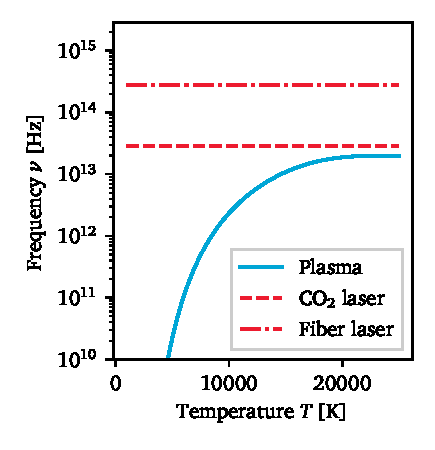
\includegraphics[]{assets/4 models/frequency_comparison}
                \caption{Comparison of plasma and laser frequencies}
                \label{fig:coulomb_freq}
            \end{subfigure}
            \hfill
            \begin{subfigure}[t]{2.9in}
                \centering
                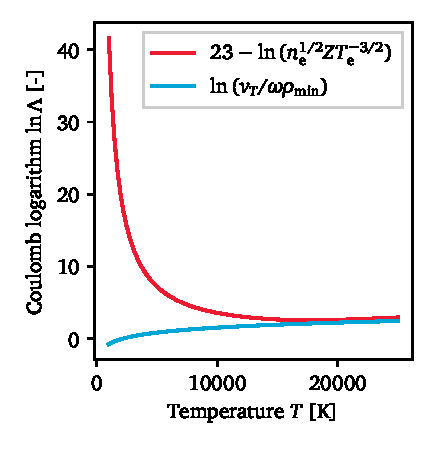
\includegraphics[]{assets/4 models/coulombLog}
                \caption{Comparison of computation methods}
                \label{fig:coulomb_coulomb}
            \end{subfigure}
            \caption{Calculation of the Coulomb logarithm, \qty{10}{bar}}
            \label{fig:coulomb}
        \end{figure}

        With values for the Coulomb logarithm and the plasma frequency, \autoref{eq:ib_absorption} can be evaluated. \autoref{fig:ib_coeff} plots the IB absorption coefficient for a range of temperatures and pressures. The point of peak absorption appears around the \num{20000}-\unit{K} mark, with a sharp rise in peak absorption coefficient with increasing pressure. This is expected as $\alpha$ is proportional to $n_\mathrm{e}^2$ on the first order, which increases with pressure. The occurrence of peak absorption appears to shift to greater temperatures as pressure increases.

        \begin{figure}[h]
            \centering
            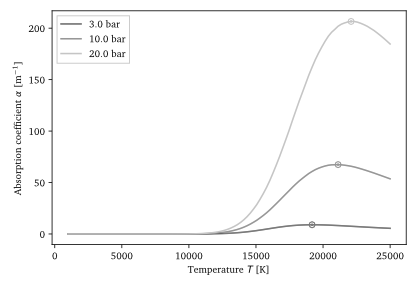
\includegraphics[]{assets/4 models/absorption}
            \caption{Inverse bremsstrahlung absorption coefficient of argon at various pressures, \num{1070}-\unit{nm} radiation}
            \label{fig:ib_coeff}
        \end{figure}

        The temperature of peak absorption is of interest, as it correlates to the peak temperature of the LSP (\textcite{keeferLaserSustainedPlasmas1989}). This absorption model thus suggests that a peak temperature of \highlight[id=BZ, comment=Later you show (...) that temperatures remain below true plasma temperatures. What are the alternative heating mechanisms?]{around \qty{20000}{K}}\comment[id=ED]{Now addressed in \autoref{sec:results_spectroscopy}} should be expected. \added{Furthermore, the calculated absorption coefficient provides a scale length over which laser radiation will be absorbed by the LSP, by taking the reciprocal of $\alpha$. For instance, at \qty{10}{bar} of pressure and assuming complete absorption, the LSP length can be estimated to be close to the absorption length, i.e., $1/(\qty{67}{m^{-1}}) =$~\qty{15}{mm}. Experimental measurements of the fraction of laser power absorbed by the LSP can be used with the measured LSP length to compute an effective absorption coefficient, which can be compared to the predicted values in \autoref{fig:ib_coeff}, using the Beer-Lambert law.}
    
    \section{LSP size estimate}
        Another avenue for LSP temperature estimate is to relate the average temperature and plasma volume, assuming the laser pulse energy is converted into enthalpy in the plasma volume. This calculation can then provide a range of LSP volumes and their associated average temperature. \autoref{fig:LSP_size_model_diagram} illustrates the simplified model of the LSP. The plasma volume is considered to be perfectly bounded by the laser beam and is approximated as a cone whose tip coincides with the laser focus. Knowing the beam geometry, i.e., the f-number $N_\mathrm{f} = 7.9$, means that the cone's volume is only a function of the LSP length $d$.
        \begin{equation}
            \frac{d}{2r} = N_\mathrm{f} \implies V = \pi\frac{d^3}{12N_\mathrm{f}^2}
        \end{equation}
        Starting with an initial temperature $T_1$ of \qty{290}{K}, a final temperature $T_2$ will correspond to a change in enthalpy $\Delta h$. Given a set pulse energy $E_\mathrm{in}$ absorbed with efficiency $\eta_\alpha$, the mass $m$ of gas required to increase in temperature from $T_1$ to $T_2$ can be found with \autoref{eq:deltahtom}:
        \begin{equation}
            m = \frac{\eta_\alpha E_\mathrm{in}}{\Delta h(T_1, T_2)} \label{eq:deltahtom}
        \end{equation}
        This mass can then be converted to a volume $V$ based on the density $\rho(T_2)$ of the gas at temperature $T_2$.

        \begin{figure}[h]
            \centering
            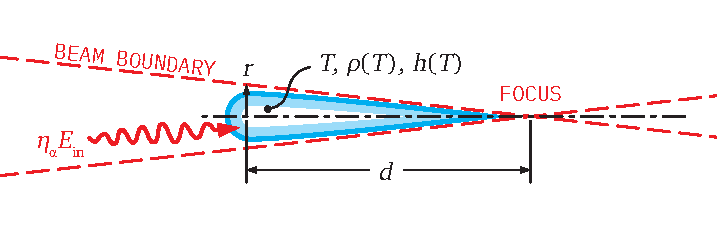
\includegraphics[]{assets/4 models/LSP_sizemodel.pdf}
            \caption{LSP sizing model}
            \label{fig:LSP_size_model_diagram}
        \end{figure}

        Unlike the heat deposition calculations discussed in the following section, the varying specific heat of argon must be considered, as it changes by an order of magnitude between 5000 and \qty{20000}{K}. At these temperatures, the ionization of argon consumes additional heat, so more of it is needed to increase its temperature. The thermodynamic properties of argon were obtained through NASA's CEA software~\cite{gordonComputerProgramCalculation1994} for a range of pressures and temperatures, and interpolated using cubic splines. The resulting specific heat at constant pressure and enthalpy are both plotted in \autoref{fig:argon_thermo} for \qty{10}{bar} of ambient pressure.

        \begin{figure}[h]
            \centering
            \begin{subfigure}[t]{0.47\textwidth}
                \centering
                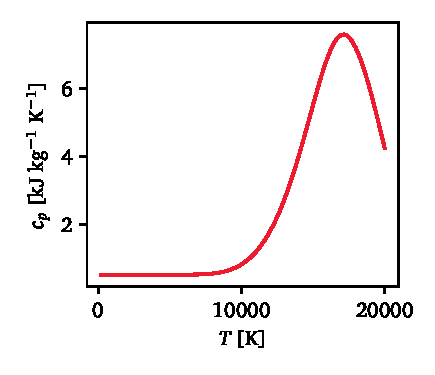
\includegraphics[width=\textwidth]{assets/4 models/Ar10_cp.pdf}
                \caption{Specific heat of enthalpy}
                \label{fig:argon_cp}
            \end{subfigure}
            \hfill
            \begin{subfigure}[t]{0.47\textwidth}
                \centering
                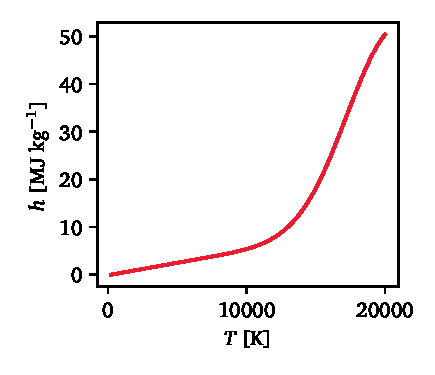
\includegraphics[width=\textwidth]{assets/4 models/Ar10_h.pdf}
                \caption{Enthalpy}
                \label{fig:argon_h}
            \end{subfigure}
            \caption{Thermodynamic properties of argon at \qty{10}{bar}}
            \label{fig:argon_thermo}
        \end{figure}

        The varying density $\rho(T)$ was also taken from CEA's output. \autoref{fig:LSP_size_model} shows the resulting LSP dimensions based on a range of possible final temperatures. The calculation was performed for two pressures and assuming both complete and 50\% laser absorption by the plasma. The results suggest that in the range where ionization is expected and IB absorption is possible, i.e., above \qty{10000}{K}, the volume of plasma that would contain the energy of a full-power pulse ranges from 10--1000~\unit{mm^3}, corresponding to LSP lengths on the order of \qty{10}{mm}. Although not a perfect match, this loosely corresponds to the scale absorption lengths suggested by the IB absorption calculation in \autoref{sec:models_absorption}, especially at higher temperatures.

        \begin{figure}[h]
            \centering
            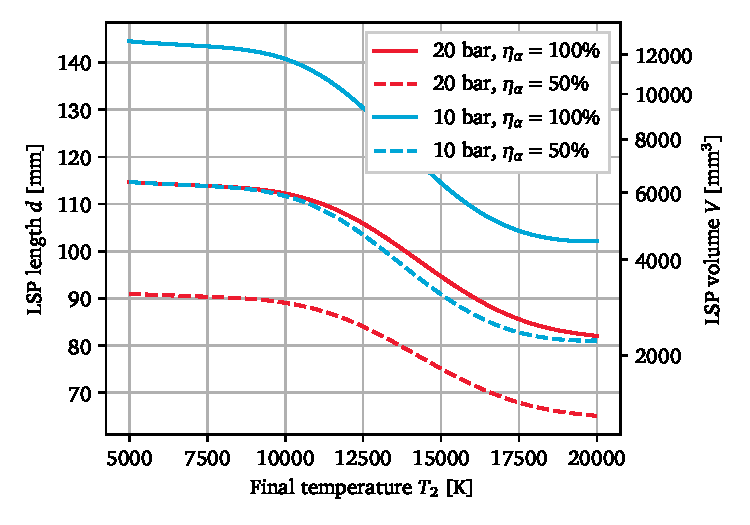
\includegraphics[]{assets/4 models/volume_est.pdf}
            \caption{LSP dimension estimate for \qty{30}{J} pulse, assuming conical volume}
            \label{fig:LSP_size_model}
        \end{figure}

        This model of LSP sizing does have a few caveats. First, it assumes that the plasma envelope is adiabatic---none of the heat deposited into the plasma is transferred out within the duration of a laser pulse. In reality, heat will likely be lost through radiation and conduction as the plasma grows. Second, the plasma temperature will not be uniform, as seen in the data from \textcite{welleEnergyConversionEfficiency1986} (\autoref{fig:4_LSPTProfile}), and a portion of the plasma will lie outside of the laser-beam boundaries. These effects will likely result in a smaller than estimated plasma volume/length, as less heat will be contained in the plasma envelope at any given time and a portion of this heat will be contained in lower-temperature regions.

    \section{Test-section heating}
        Some calculations were performed in the interest of safety and selecting appropriate instrumentation to predict the rise in temperature and pressure of the test section during an experiment. As discussed in \autoref{sec:design_pressuresensor}, precise pressure measurements will be taken during the experiment to estimate the heat deposition resulting from successful LSP ignition. The following scenarios are considered:
        \begin{enumerate}
            \item Failed ignition
            \item Successful ignition
            \begin{enumerate}
                \item ...in the static case (constant volume)
                \item ...in the flowing case (constant pressure)
            \end{enumerate}
        \end{enumerate}
        The apparatus used in this project is mostly made of stainless steel and 6061~aluminum, and argon is the working fluid. Some relevant thermodynamic and structural properties are given in \autoref{chp:app_matprops}.

        \subsection{Failed ignition}
            In the case of failed ignition, most of the laser radiation will be directly incident on the backplate of the test section. This is the worst case scenario---alternatively, a window module could be present, allowing the laser beam to be safely dumped into the power meter, resulting in virtually no heating of the test section itself. The opaque backplate used in this experiment is made of 6061 aluminum. It can be approximated as a disk \qty{3.94}{in} in diameter and 0.39-in thick, giving it a mass of approximately \qty{0.2}{kg} and a heat capacity of \qty{180}{J.K^{-1}}. The worst-case temperature rise can be estimated assuming all the laser energy is absorbed by the plate as heat.

            It is immediately apparent that distributing the energy of a full-power laser pulse (\qty{30.8}{J}) will lead to a negligible temperature rise---less than \qty{0.2}{K}. The portion of the plate directly exposed to the laser beam will likely experience a higher temperature, but the beam diameter is approximately \qty{2}{cm} by the time it reaches the backplate, so local laser intensity will not be sufficient to cause any damage or to raise the surface temperature by more than a few K. In the CW scenario, with up to \qty{350}{W} deposited into the plate, the plate temperature is unlikely to rise by more than 10--20~K in the time it would take to determine that no ignition had occurred and to shut down the laser, i.e., around 10~s.

            In reality, the resulting temperature rise is likely to be much lower, as aluminum will reflect most of the laser radiation: \textcite{pozzobonHouseholdAluminumFoil2020} reported 96--98\% reflectivity in the near-infrared spectrum. The diffuse reflection (up to 75\%) will distribute the laser radiation across several parts of the apparatus, minimizing local temperature rises. Laser damage to the facility in the event of a failed ignition is thus of minimal concern.

        \subsection{Successful ignition}
            In the case of successful ignition, several scenarios are possible depending on whether the laser is operated in pulsed or CW mode and whether the working fluid is static or flowing through the test section. Two scenarios will be considered: the effect of a laser-pulse-sustained plasma in static argon, as it is the most relevant to the experiments performed in this project, and the effect of continuous LSP in flowing argon, as this is the scenario most relevant to operating a thruster prototype.

            % The use of maximum power/energy settings (i.e., \qty{350}{W}/\qty{30.8}{J}) is assumed, and calculations will be performed assuming 10\% and 100\% heat deposition efficiencies.

            \subsubsection*{Laser-pulse LSP in static argon}\comment[id=ED]{A large part of this subsubsection was originally in Chapter 5}
                Assuming an even distribution of heat added into a closed system, the resulting pressure change $\Delta p$ can be expressed using the ideal gas equation and the change in temperature $\Delta T$ caused by a constant volume heat addition $Q_\mathrm{in}$. In this case, $Q_\mathrm{in}$ refers to the heat deposition in the working fluid, not the laser-pulse energy entering the test section, which will be defined as $E_\mathrm{in}$. 
                \begin{gather}
                    pV = mR_\mathrm{g}T \label{eq:IGL}\\
                    Q_\mathrm{in} = mc_V\Delta T \label{eq:cvHeatAdd}
                \end{gather}
                The change in pressure and temperature of this system can be determined between two states (1 and 2) as follows:
                \begin{gather*}
                    \frac{p_1}{T_1} = \frac{mR_\mathrm{g}}{V} = \frac{p_2}{T_2} \\
                    \implies \frac{T_2}{T_1} = \frac{p_2}{p_1} \\
                    \implies \frac{T_1+\Delta T}{T_1} = \frac{p_1+\Delta p}{p_1} \\
                    \implies \frac{\Delta T}{T_1} = \frac{\Delta p}{p_1} \\
                    \implies \frac{p_1}{T_1}\Delta T = \Delta p
                \end{gather*}
                Substituting $p_1/T_1$ with \autoref{eq:IGL} and $\Delta T$ with \autoref{eq:cvHeatAdd}, the static pressure change in the test section can be related to the heat added in the system and vice-versa:
                \begin{equation}
                    \Delta p = \frac{R_\mathrm{g}Q_\mathrm{in}}{Vc_V}
                \end{equation}
                \added{The specific heat at constant volume $c_V$ is taken to be that of room-temperature-and-pressure argon: \qty{312}{J.kg^{-1}.K^{-1}}~\cite{lemmonThermophysicalPropertiesFluid2023}. Although the specific heats of argon vary significantly as it heats to a plasma state, this analysis considers the final state of the system, whose temperature is not expected to increase to a point where variable specific heats should be considered. }The resulting change in pressure is independent of the gas mass, and therefore, independent of the initial pressure for a set volume. This \added{initial-pressure independence }however \deleted{would} only hold\added{s} as long as the heat deposited in the gas $Q_\mathrm{in}$ is also independent on the initial pressure.

                The heat-deposition efficiency can then be defined as $\eta = Q_\mathrm{in}/E_\mathrm{in}$. Approximating the volume $V$ of the test-section as a cylinder matching the internal dimensions annotated in \autoref{fig:cavitation_dimensions} (315$\times$38-\unit{mm} cylinder) allows the prediction of the measured pressure change resulting from an LSP test. These results are shown for a range of laser-pulse energies in \autoref{fig:heatdep_p_static}. Although the pressure rise is independent of the initial pressure, the temperature rise is not. Indeed, lower initial pressures result in a lesser gas mass to absorb the deposited heat, resulting in a greater final temperature. As seen in \autoref{fig:heatdep_T_static}, the same pulse providing a $\sim$1-K temperature rise at \qty{20}{bar} would raise the temperature by almost \qty{10}{K} at \qty{3}{bar}.

                Two assumptions made in this model may not be accurate. First, this model assumes that the heat deposited by the LSP in the working gas is distributed evenly in the test section before it has time to be transferred to the test section walls. This may not be the case, so numerical simulations may be necessary to ascertain the validity of this assumption. Second, this model assumes that the heat-deposition efficiency does not change with pressure/density, when a denser gas could contribute to improved heat deposition through more effective heat conduction and/or greater absorption of radiated heat.

                The predicted state changes for this experiment are still low when considering thrust applications. As will be discussed in \autoref{sec:model_thrust}, both thrust and specific impulse depend on $T^{1/2}$. In case of low heat-deposition efficiency, a temperature change of a few K will likely only modify thrust and specific impulse by a few \% or less from the cold-flow case. It is thus already apparent that the current test-section design is unoptimized for thruster experiments, and these calculations indicate that thrust chamber volume should be decreased to amplify the changes in pressure and temperature during LSP operation.

                \begin{figure}[h]
                    \centering
                    \begin{subfigure}[t]{0.49\textwidth}
                        \centering
                        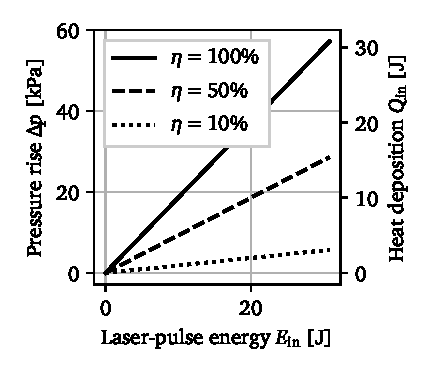
\includegraphics[]{assets/4 models/heatdep_static.pdf}
                        \caption{Resulting pressure rise}
                        \label{fig:heatdep_p_static}
                    \end{subfigure}
                    \hfill
                    \begin{subfigure}[t]{0.49\textwidth}
                        \centering
                        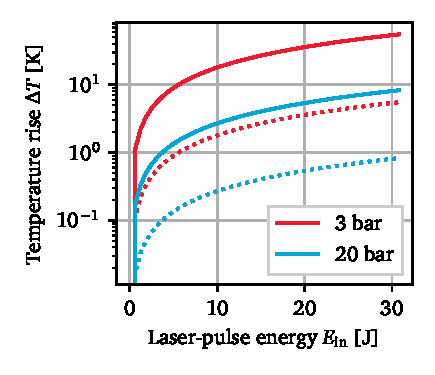
\includegraphics[]{assets/4 models/heatdep_T_static.pdf}
                        \caption{Temperature rise dependency on initial pressure}
                        \label{fig:heatdep_T_static}
                    \end{subfigure}
                    \caption{Effect of pulse LSP on test-section conditions}
                    \label{fig:heatdep_static}
                \end{figure}

            \subsubsection*{CW LSP in flowing argon}
                The CW flowing case is most akin to a real thruster operation. In this scenario, the resulting steady-flow temperature rise can be calculated for a range of mass-flow rates and a constant laser power input of \qty{350}{W}. This is a constant-pressure process, unlike the static LSP case. For steady flow, the temperature change from $T_1$ (room temperature) to $T_2$ due to a heat addition rate $\dot{Q}_\mathrm{in}$ can be determined from its change of enthalpy as follows:
                \begin{equation}
                    \eta P_\mathrm{in} = \dot{Q}_\mathrm{in} = \dot{m}(h(T_2)-h(T_1))
                \end{equation}
                Where $P_\mathrm{in}$ is the laser power and $\eta$ is the heat-deposition efficiency. This equation can be solved for $T_2$, the resulting bulk temperature at the inlet of the thruster nozzle. Again, variable specific heat data from NASA CEA~\cite{gordonComputerProgramCalculation1994} will be considered to determine what mass flow rates are necessary to attain temperatures expected in an actual LTP system, i.e., 10$^3$--10$^4$~K.

                \autoref{fig:heatdep_flowing} shows the result of this calculation for mass-flow rates ranging from 0.03 to \qty{30}{g.s^{-1}} and a chamber pressure of \qty{10}{bar}. At this low laser-power level, low mass-flow rates of \qty{1}{g.s^{-1}} or less appear necessary to raise the propellant temperature to those expected in an LTP thruster. In the best case conditions, the theoretical 10~000-K chamber temperature reported by \textcite{duplayDesignRapidTransit2022} for a full-scale thruster can only be replicated in the lab with a 0.06-\unit{g.s^{-1}} flow rate. Temperature increases appear negligible for flow rates beyond \qty{20}{g.s^{-1}}.

                \begin{figure}[h]
                    \centering
                    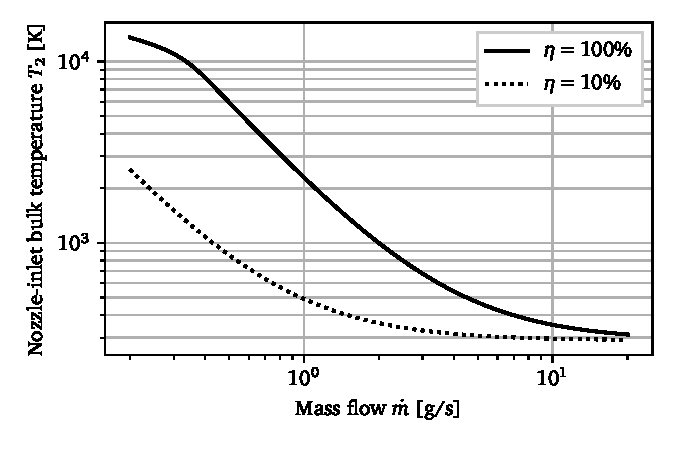
\includegraphics[]{assets/4 models/heat_addition_flowing.pdf}
                    \caption[Expected flow temperature at nozzle inlet]{Expected flow temperature at nozzle inlet, \qty{10}{bar}, \qty{350}{W} of input laser power.}
                    \label{fig:heatdep_flowing}
                \end{figure}
    
    \section{Thrust modelling} \label{sec:model_thrust}
        Sizing thruster and thrust-stand components requires the calculation of theoretical performance parameters such as the expected thrust and exhaust velocity. These parameters should be calculated for a range of operating conditions, which include the chamber pressure, the laser power, and the mass flow rate. Given the number of factors affecting thrust, a complete study of the operating range and theoretical performance of a prototype thruster could be the subject of its own thesis. Therefore, three specific scenarios (tabulated in \autoref{tab:thruster_scenarios}) will be studied in detail:
        \begin{itemize}
            \item \textbf{CW20:} CW laser input at maximum power (\qty{350}{W}). At this power level, the minimum pressure allowing a stable LSP is \qty{20}{bar} according to \textcite{zimakovInteractionNearIRLaser2016}. This is thus the only operating scenario in which the LTTLM could be operated continuously.
            \item \textbf{P20:} Full-power (\qty{3080}{W}) laser pulse generating LSP at \qty{20}{bar}.
            \item \textbf{P3:} At \qty{3}{bar}, the LSP power threshold is approximately \qty{3}{kW}. This is the lowest pressure at which the LTTLM could theoretically be operated with the available laser.
        \end{itemize}

        \begin{table}[h]
            \centering
            \caption[Operating scenarios for the LTTLM]{Operating scenarios for the LTTLM, $p_{\mathrm{c,}1}$ is the initial chamber pressure and $\dot{Q}_\mathrm{in}$ is the input power.}
            \label{tab:thruster_scenarios}
            \begin{tabular}{@{}lrrl@{}}
                \toprule
                Scenario    & $p_{\mathrm{c,}1}$ [\unit{bar}]  & $\dot{Q}_\mathrm{in}$ [W] & Laser mode \\
                \midrule
                CW20    & 20    &  350  & CW \\
                P20     & 20    & 3080  & Pulsed \\
                P3      &  3    & 3080  & Pulsed \\
                \bottomrule
            \end{tabular}
        \end{table}

        The thrust $F_\mathrm{T}$ of a thermal rocket engine can be determined with \autoref{eq:thrust}, where $T_\mathrm{c}$ is the chamber temperature, $p_\mathrm{ex}$ is the exhaust pressure, $p_\mathrm{c}$ is the chamber pressure, $A_\mathrm{ex}$ is the nozzle exit area, and $p_\mathrm{a}$ is the ambient pressure.
        \begin{equation}
            F_\mathrm{T} = \dot{m}\sqrt{\frac{2\gamma}{\gamma-1}R_\mathrm{g}T_\mathrm{c}\left(1-\left(\frac{p_\mathrm{ex}}{p_\mathrm{c}}\right)^\frac{\gamma-1}{\gamma}\right)} + A_\mathrm{ex}(p_\mathrm{ex}-p_\mathrm{a}) \label{eq:thrust}
        \end{equation}
        In this case, the thruster will exhaust to atmosphere, so $p_\mathrm{a}$ will be set to \qty{1}{bar}. The following simplifying assumptions will also be made:
        \begin{enumerate}
            \item The mass-flow rate $\dot{m}$ into the thruster will be held constant. This is achievable in practice by setting up the system in a \emph{double-choked} configuration, where the inlet port is a choked orifice whose mass-flow rate is only dependent on upstream stagnation conditions.
            % $p_0$ and $T_0$:
                % \[\dot{m} = K_{\dot{m}}A_\mathrm{t}\frac{p_0}{\sqrt{T_0}}\]
                The flow can then choke again at the thruster's nozzle throat, provided a normal shock occurs between the inlet port and the thrust chamber. For the sake of brevity, a complete flow analysis will not be given, but this configuration is theoretically possible and is considered for the next iteration of the LTTLM, which is in development at the time of writing this report.
            \item The thruster nozzle will be assumed to be a simple orifice with no diverging section, meaning that the exit pressure $p_\mathrm{ex}$ is equal to the flow's sonic pressure $p^*$, i.e., the pressure of the flow as it reaches sonic conditions. The sonic pressure is a function of stagnation pressure $p_\mathrm{c}$ and the specific heat ratio $\gamma$ of the gas:
            \begin{equation}p^* = p_\mathrm{c}\left(\frac{2}{\gamma+1}\right)^\frac{\gamma}{\gamma-1} \approx 0.5p_\mathrm{c}\;\text{(Argon)}\label{eq:sonicpressure}\end{equation}
            The choked orifice is the simplest, albeit unoptimized, nozzle configuration. Adding a diverging section would not fundamentally change the flow conditions in the thruster; it would merely improve thrust and specific impulse.
            \item Finally, argon will be treated as a perfect gas, i.e., $c_p$ and $\gamma$ are constant. This is a valid assumption for argon until $\sim$\qty{5000}{K}~\cite{gordonComputerProgramCalculation1994}. As the intent of the LTTLM is not yet to attain such high temperatures, this is a suitable simplification.
        \end{enumerate}

        \subsection{Cold-flow conditions}
            Starting the thruster will involve a cold-thrust stage (denoted with the subscript 1) before the laser is turned on. Flow conditions should stabilize such that the desired chamber pressure is attained. In this case, the chamber temperature remains close to room temperature $T_\mathrm{a}$ (\qty{290}{K}). For a desired mass-flow rate and chamber pressure, the nozzle exit area (i.e., the orifice size) is fully constrained by the \autoref{eq:massflow}\footnote{Equivalent to Equation 6-6 in \citeauthor{zandbergenAE4S01ThermalRocket2020}'s \citetitle*{zandbergenAE4S01ThermalRocket2020} course notes~\cite{zandbergenAE4S01ThermalRocket2020}} for the choked mass-flow rate.\comment[id=ED]{Moved from \autoref{sec:exp_flowing}}
            \begin{equation} 
                \dot{m} = \sqrt{\frac{\gamma}{R_\mathrm{g}}\left(\frac{2}{\gamma+1}\right)^\frac{\gamma+1}{\gamma-1}}\frac{A_\mathrm{ex}p_\mathrm{c}}{\sqrt{T_\mathrm{c}}} = K_{\dot{m}}\frac{A_\mathrm{ex}p_\mathrm{c}}{\sqrt{T_\mathrm{c}}} \label{eq:massflow}
            \end{equation}
            \begin{equation*}
                \implies A_\mathrm{ex} = \frac{\dot{m}}{K_{\dot{m}}}\frac{\sqrt{T_\mathrm{a}}}{p_\mathrm{c,1}}
            \end{equation*}
            For the temperatures of interest in the overall flow (excluding the LSP), $K_{\dot{m}}$ for argon is \qty{0.0504}{s.K^{1/2}.m^{-1}}. \added{For those familiar with the Vandenkerckhove function $\Gamma$, the mass flow parameter $K_{\dot{m}}$ is equivalent to $\Gamma/R_\mathrm{g}^{1/2}$.}

            The orifice area $A_\mathrm{ex}$ is then assumed to remain constant throughout both cold-flow and hot-fire conditions---no variable geometry nozzles are currently planned for the thruster prototype. The thrust equation \autoref{eq:thrust} can now be evaluated for cold flow conditions. \autoref{fig:cold_thrust} shows the variation in thrust and the nozzle dimension for a mass-flow rate ranging from 1--10~\unit{g.s^{-1}}. The cold thrust appears to remain on the order of \qty{1}{N} regardless of chamber pressure, though the difference between \qty{3}{bar} and \qty{20}{bar} appears to grow at greater mass-flow rates. The nozzle diameter exhibits a more significant difference between both chamber pressures. It should be noted that the CW20 and P20 scenarios are perfectly superposed---this is normal since the only difference between both cases is the laser power, which is not active at this stage.

            \begin{figure}[h]
                \centering
                \begin{subfigure}[t]{0.48\textwidth}
                    \centering
                    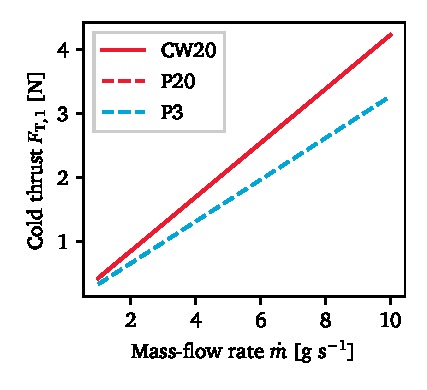
\includegraphics[width=\textwidth]{assets/4 models/cold_thrust.pdf}
                    \caption{Thrust}
                    \label{fig:cold_thrust_thrust}
                \end{subfigure}
                \hfill
                \begin{subfigure}[t]{0.48\textwidth}
                    \centering
                    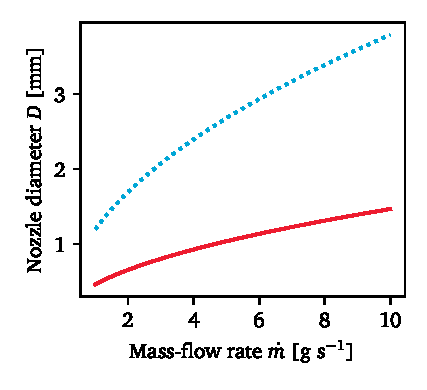
\includegraphics[width=\textwidth]{assets/4 models/cold_thrust_nozzle.pdf}
                    \caption{Nozzle diameter}
                    \label{fig:cold_thrust_nozzle}
                \end{subfigure}
                \caption[Cold gas thruster parameters]{Cold gas thruster parameters. Legend is shared between both plots.}
                \label{fig:cold_thrust}
            \end{figure}

            Although the thrust increases with $\dot{m}$, the exhaust velocity $v_\mathrm{ex}$ is unaffected by the mass-flow rate---its value for each scenario is tabulated in \autoref{tab:cold_vexhaust}. The equivalent exhaust velocity $v_\mathrm{eq}$ is also is given. This term combines the true exhaust velocity with the pressure thrust $A_\mathrm{ex}\Delta p_{ex-a}$ normalized by mass-flow rate. The equivalent exhaust velocity is commonly used to simplify calculations for rocket trajectories and mission planning, as no special attention must be given to pressure-thrust effects. The specific impulse $I_\mathrm{sp}$ is also commonly used to report rocket engine exhaust velocities. These various forms of expressing the exhaust velocity are related by the following equations:
            \begin{gather*}
                F_\mathrm{T} = \dot{m}v_\mathrm{ex} + A_\mathrm{ex}(p_\mathrm{ex}-p_\mathrm{a}) \\
                v_\mathrm{eq} = v_\mathrm{ex} + \frac{A_\mathrm{ex}(p_\mathrm{ex}-p_\mathrm{a})}{\dot{m}} \\
                I_\mathrm{sp} = \frac{v_\mathrm{eq}}{g_0} \\
                \implies F_\mathrm{T} = \dot{m}v_\mathrm{eq} = \dot{m}I_\mathrm{sp}g_0
            \end{gather*}
            Where $g_0$ is the standard gravitational acceleration. For the rest of this analysis, the \emph{equivalent} exhaust velocity $v_\mathrm{eq}$ will be reported, as the true exhaust velocity is of lesser interest.

            \begin{table}[h]
                \centering
                \caption[Cold-flow exhaust velocities]{Cold-flow (stage 1) exhaust velocities: $v_\mathrm{ex}$ is the real exit flow velocity, $v_\mathrm{eq}$ is the equivalent exhaust velocity, and $I_\mathrm{sp}$ is the specific impulse based on $v_\mathrm{eq}$.}
                \label{tab:cold_vexhaust}
                \begin{tabular}{@{}lrrr@{}}
                    \toprule
                    Scenario    & $v_\mathrm{ex,1}$ [\unit{m.s^{-1}}] & $v_\mathrm{eq,1}$ [\unit{m.s^{-1}}] & $I_\mathrm{sp,1}$ [s] \\
                    \midrule
                    CW20    & 275   &  422  & 43 \\
                    P20     & 275   &  422  & 43 \\
                    P3      & 275   &  327  & 33 \\
                    \bottomrule
                \end{tabular}
            \end{table}

            Again, there is no difference in the resulting exhaust velocity between the CW20 and P20 scenarios. This is not surprising considering the chamber pressure is identical, and the use of an orifice nozzle means that the $p_\mathrm{ex}/p_\mathrm{c}$ ratio reduces to a function of $\gamma$, which is identical in both cases. P3 yields a lesser equivalent exhaust velocity than the other two scenarios as the pressure thrust is decreased.

        \subsection{Hot-fire conditions}
            Once cold-flow conditions have been established, the laser is turned on and LSP is assumed to be ignited successfully. The flow is expected to adjust to the heat addition, resulting in new, hot-fire flow conditions (stage 2). The heat deposition is assumed to be 100\% efficient and results in a change in chamber temperature as modelled in \autoref{eq:heatdep}. The perfect gas assumption does simplify the model as follows:
            \begin{equation}
                T_\mathrm{c,2} = T_\mathrm{c,1} + \frac{\dot{Q}_\mathrm{in}}{\dot{m}c_p}
            \end{equation}
            Where $T_\mathrm{c,1}$ is the chamber temperature in state 1, i.e., $T_\mathrm{a}$.

            Under the assumed constant mass-flow rate conditions, this increase in temperature must lead to an increase in chamber pressure $p_\mathrm{c}$. Indeed, by examining conservation of mass:
            \begin{align*}
                \dot{m}_1 &= \dot{m}_2 \\
                \implies K_{\dot{m}}\frac{A_\mathrm{ex}p_\mathrm{c,1}}{\sqrt{T_\mathrm{c,1}}} &= K_{\dot{m}}\frac{A_\mathrm{ex}p_\mathrm{c,2}}{\sqrt{T_\mathrm{c,2}}} \\
                \implies \frac{p_\mathrm{c,1}}{\sqrt{T_\mathrm{c,1}}} &= \frac{p_\mathrm{c,2}}{\sqrt{T_\mathrm{c,2}}}
            \end{align*}
            Since the nozzle area cannot be changed, the only way to maintain the same mass flow is to increase the chamber pressure. \autoref{fig:change_hotThrust_Tp} shows the new chamber temperature and the change in chamber pressure resulting from the heat addition. The chamber temperature is in good agreement with \autoref{fig:heatdep_flowing}, where variable specific heat was considered. Here, both P20 and P3 are perfectly superposed, as they share the same rate of heat addition. Since the increase in temperature is dependent on the mass-flow rate, the order-of-magnitude difference in input power between the CW and pulsed laser results in a similar difference in chamber temperature.

            \begin{figure}[h]
                \centering
                \begin{subfigure}[t]{0.48\textwidth}
                    \centering
                    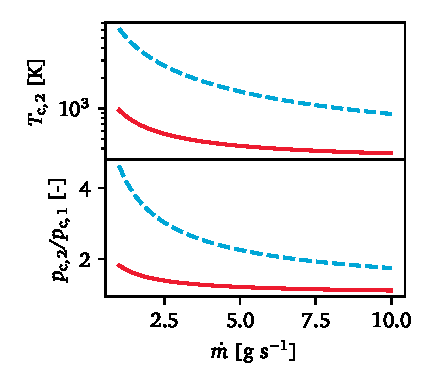
\includegraphics[width=\textwidth]{assets/4 models/thermo_hotThrust.pdf}
                    \caption{Chamber temperature and change in pressure}
                    \label{fig:change_hotThrust_Tp}
                \end{subfigure}
                \hfil
                \begin{subfigure}[t]{0.48\textwidth}
                    \centering
                    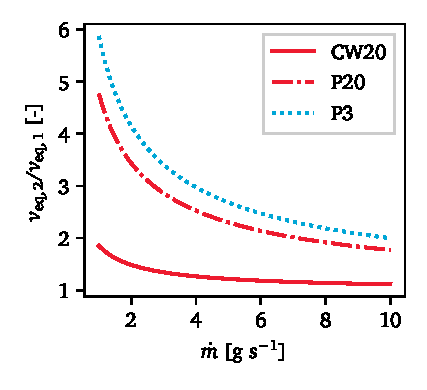
\includegraphics[width=\textwidth]{assets/4 models/veRatio_hotThrust.pdf}
                    \caption{Ratio of equivalent exhaust velocity}
                    \label{fig:change_hotThrust_veRatio}
                \end{subfigure}
                \caption[Change in operating parameters between cold (1) and hot (2) flow]{Change in operating parameters between cold (1) and hot (2) flow. Legend is shared.}
                \label{fig:change_hotThrust}
            \end{figure}

            The change in pressure is also significant. A two-fold increase in chamber pressure is observed for a 3-kW input power (P20 and P3) at a 10-\unit{g.s^{-1}}-mass-flow rate, and this pressure ratio increases to above 4 at \qty{1}{g.s^{-1}}. The CW20 case approaches a two-fold increase in pressure at \qty{1}{g.s^{-1}}. This has major implications in the thrust-chamber design: in the P20 and CW20 case, this would mean an operating pressure of around \qty{80}{bar} and \qty{40}{bar}, respectively---significantly greater than the current test section's design pressure. Furthermore, in order to maintain a constant mass-flow rate at the inlet port, the chamber pressure \emph{must} remain below the reservoir's sonic pressure, i.e., around half of the reservoir's stagnation pressure (\autoref{eq:sonicpressure}). This suggests that unless the feed system can be designed to respond to this pressure change, the reservoir's pressure should be an order of magnitude greater than the cold-flow operating pressure $p_\mathrm{c,1}$. The increase in chamber pressure does have a benefit: this moves the thruster operating point further beyond the LSP power threshold, which should facilitate the maintenance of the plasma.

            The change in exhaust velocity is shown in \autoref{fig:change_hotThrust_veRatio}. Although P20 and P3 exhibit the same relative pressure change and have the same $T_\mathrm{c,2}$, a greater relative change in exhaust velocity is observed in the P3 scenario. This is due to a difference in pressure thrust: since P3 uses a larger nozzle for a given mass-flow rate (as seen in \autoref{fig:cold_thrust_nozzle}), the contribution of the pressure thrust to the equivalent exhaust velocity is proportionally greater. The CW20 scenario exhibits a change in exhaust velocity that mirrors its change in chamber pressure. The use of equivalent exhaust velocity over the real exhaust velocity is convenient here: since the thrust is directly proportional to $v_\mathrm{eq}$, the relative change in equivalent exhaust velocity is the same as the relative change in thrust $F_\mathrm{T,2}/F_\mathrm{T,1}$.

            \autoref{fig:thruster_perf} shows the final thrust performance figures of an LTP thruster model powered by the laser used in this project. Ultimately, the thruster-operation mode described here makes a change in pressure from \qtyrange{3}{20}{bar} unimportant compared to a difference in power input: both the P20 and P3 scenarios have similar thrust levels across the given mass-flow-rate range (although, again, the difference grows at greater $\dot{m}$). Although noticeably lower, the thrust level of the CW20 scenario is still somewhat comparable: all three scenarios result in thrust on the order of \qty{1}{N}. Detecting a noticeable change in exhaust velocity and/or thrust between cold and hot flow will however require mass-flow rates closer to \qty{1}{g.s^{-1}}. The expected exhaust velocities range from \qty{500}{m.s^{-1}} for the CW20 case to up to \qty{2}{km.s^{-1}} for the pulse-laser cases. Here again, the pressure difference between P3 and P20 result in only a minor change in exhaust velocity.

            \begin{figure}[h]
                \centering
                \begin{subfigure}[t]{0.48\textwidth}
                    \centering
                    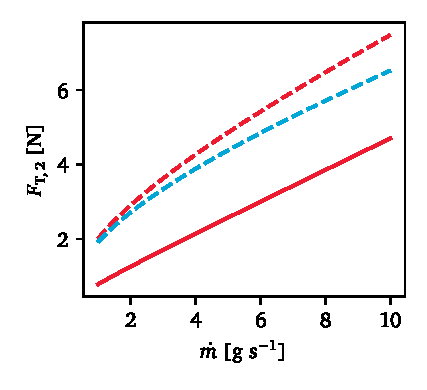
\includegraphics[width=\textwidth]{assets/4 models/thrust_hotThrust.pdf}
                    \caption{Thrust}
                    \label{fig:thruster_perf_thrust}
                \end{subfigure}
                \hfill
                \begin{subfigure}[t]{0.48\textwidth}
                    \centering
                    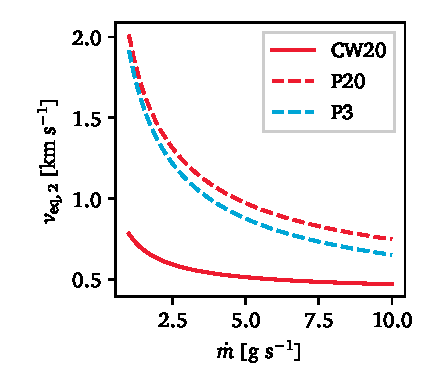
\includegraphics[width=\textwidth]{assets/4 models/ve_hotThrust.pdf}
                    \caption{Exhaust velocity}
                    \label{fig:thruster_perf_ve}
                \end{subfigure}
                \caption{Thrust and exhaust velocity, hot-fire conditions}
                \label{fig:thruster_perf}
            \end{figure}

        \subsection{Limitations}
            Although this analysis provides some valuable insight into the possible operation of a lab-scale LTP thruster and yields concrete performance estimates, the validity of its assumptions must be discussed to determine to what degree these performance predictions will apply to real tests. The most questionable assumption is likely the 100\% heat-deposition efficiency from the laser to the working fluid. The thruster tests of \textcite{toyodaThrustPerformanceCW2002} suggest that a far lesser heat-deposition efficiency is to be expected in real-world conditions, likely due to significant radiative heat losses to the thruster walls. The use of regenerative cooling could potentially alleviate this issue, but the use of more aggressive heat retention methods, such as gas seeding proposed by \textcite{shojiPerformanceHeatTransfer1976}, may be required to approach this idealized heat-deposition efficiency. If the difference in operating parameters between the P20 and CW20 scenarios is indicative, an order-of-magnitude reduction in exhaust velocity could be expected, along with a $\sim$50\% reduction in thrust. This analysis also does not consider boundary-layer effects, which may be significant based on the expected nozzle sizes---one of their potential effects is an effective reduction in the nozzle area, leading to a greater pressure than expected to achieve the same mass-flow rate.

            The P20 and P3 cases are also idealized in the sense that these calculations assume that a steady flow and heat transfer is established within the span of a 10-ms laser pulse, which is unlikely. Studying these cases does provide some understanding of the effect of increased laser power compared to the CW case, which should be analogous to a difference in heat-deposition efficiency. The CW20 case remains the most representative scenario for thrust testing.

            The takeaway from this analysis is that a well-sized load-cell should likely have a minimum resolution on the order of \qty{0.01}{N} and a maximum load rating of around \qty{1}{N}, much lower than the 10--\qty{20}{N} stated in the TS-2 thrust-stand requirement (\autoref{tab:tsReq}). This was a preliminary requirement set to allow for the use of relatively large nozzles, larger than necessary for dedicated thrust testing. As discussed in \autoref{sec:exp_flowing}, these larger nozzles allowed for bulk flow velocities in the test-section high enough to affect the LSP. In addition, as the project progressed, it quickly became apparent that the selected test-section was unoptimized for thrust testing, as its mass made it difficult to design a thrust stand that could appropriately measure its thrust. The requirements were thus not revised following in-depth thrust modelling. The analysis presented here will however inform the design of a dedicated LTP thruster model and thrust stand, in development at the time of writing.